\chapter{Profiling}

\begin{definitionbox}{Event}
    A change in the state of the system.
    \begin{itemize}
        \item Usually some granularity limit is used (e.g clock tick)
        \item Optionally has a payload (properties describing the event - e.g cache line evicted $\to$ the addresses \& data evicted)
        \item Has an accuracy - degree to which the event represents reality (many events are numeric \& come with measurement related error)
    \end{itemize}
    \begin{center}
        \begin{tabular}{l p{.8\textwidth}}
            \textbf{Simple/Atomic Event} & Executed instruction, clock tick, function called \\
            \textbf{Complex Event} & Cache line evicted, ROB flush due to misspeculation \\
        \end{tabular}
    \end{center}
    Event sources have two components:
    \begin{center}
        \begin{tabular}{l p{.8\textwidth}}
            \textbf{Generator} & Observes changes to system state (online $\to$ part of the runtime system) \\
            \textbf{Consumer} & Processes events and converts into meaningful insights (offline or online)
        \end{tabular}
    \end{center}
    The overhead associated with collecting events can be very high.
\end{definitionbox}

\begin{definitionbox}{Pertubation}
    The effect of analysis on the performance of a system.
    \begin{itemize}
        \item If it is constant/deterministic we can subtract it from measurement to get an accurate result.
        \item Non-deterministic pertubation negatively affects accuracy as it cannot separate analysis overhead from measured performance
    \end{itemize}
\end{definitionbox}

\begin{examplebox}{Stacking up!}
    Instrumentation is added to a program to inspect its stack at regular intervals, and record 
    the stack trace. Assuming it is implemented to ensure the time spent traversing the trace is 
    deterministic and can be removed from any results, why may this instrumentation still result 
    in non-deterministic pertubation?
    \tcblower
    \textbf{Data Cache Side Effects}
    \\ The instrumentation may bring \textit{deep} parts of the stack  (\textit{shallow} is \textit{hot} and likely cached) into cache, evicting other lines.
    Hence the tracing \textit{pollutes} the cache and results in more misses \& hence more memory related stalls for the program.
    \\
    \\ We could also more weakly argue about instruction cache limitations, or potential for associativity conflicts occurring may have been avoided by design in the original program, but due to placement of instrumentation's static data \& text have their positions moved.
\end{examplebox}

\begin{definitionbox}{Fidelity}
    The level of granularity with which events are recorded.
    \begin{itemize}
        \item Perfect fidelity means every event is recorded.
        \item Lower fidelity generally means less overhead.
    \end{itemize}
\end{definitionbox}

\begin{definitionbox}{Trace}
    A complete log of the system's state (and hence changes in state/events) for some time period.
    \begin{itemize}
        \item Events usually totally ordered (exceptions being with parallelism - i.e multicore systems)
        \item Accuracy is inherited from events (e.g accuracy of clock, hardware counters etc)
        \item Analysing traces is time consuming (solution: Profiling)
    \end{itemize}
\end{definitionbox}

Events may be aggregated to reduce the logging overhead.

\subsection{Call Stack Tracing}
A common trace is to capture and inspect the stack of a thread.
\begin{center}
    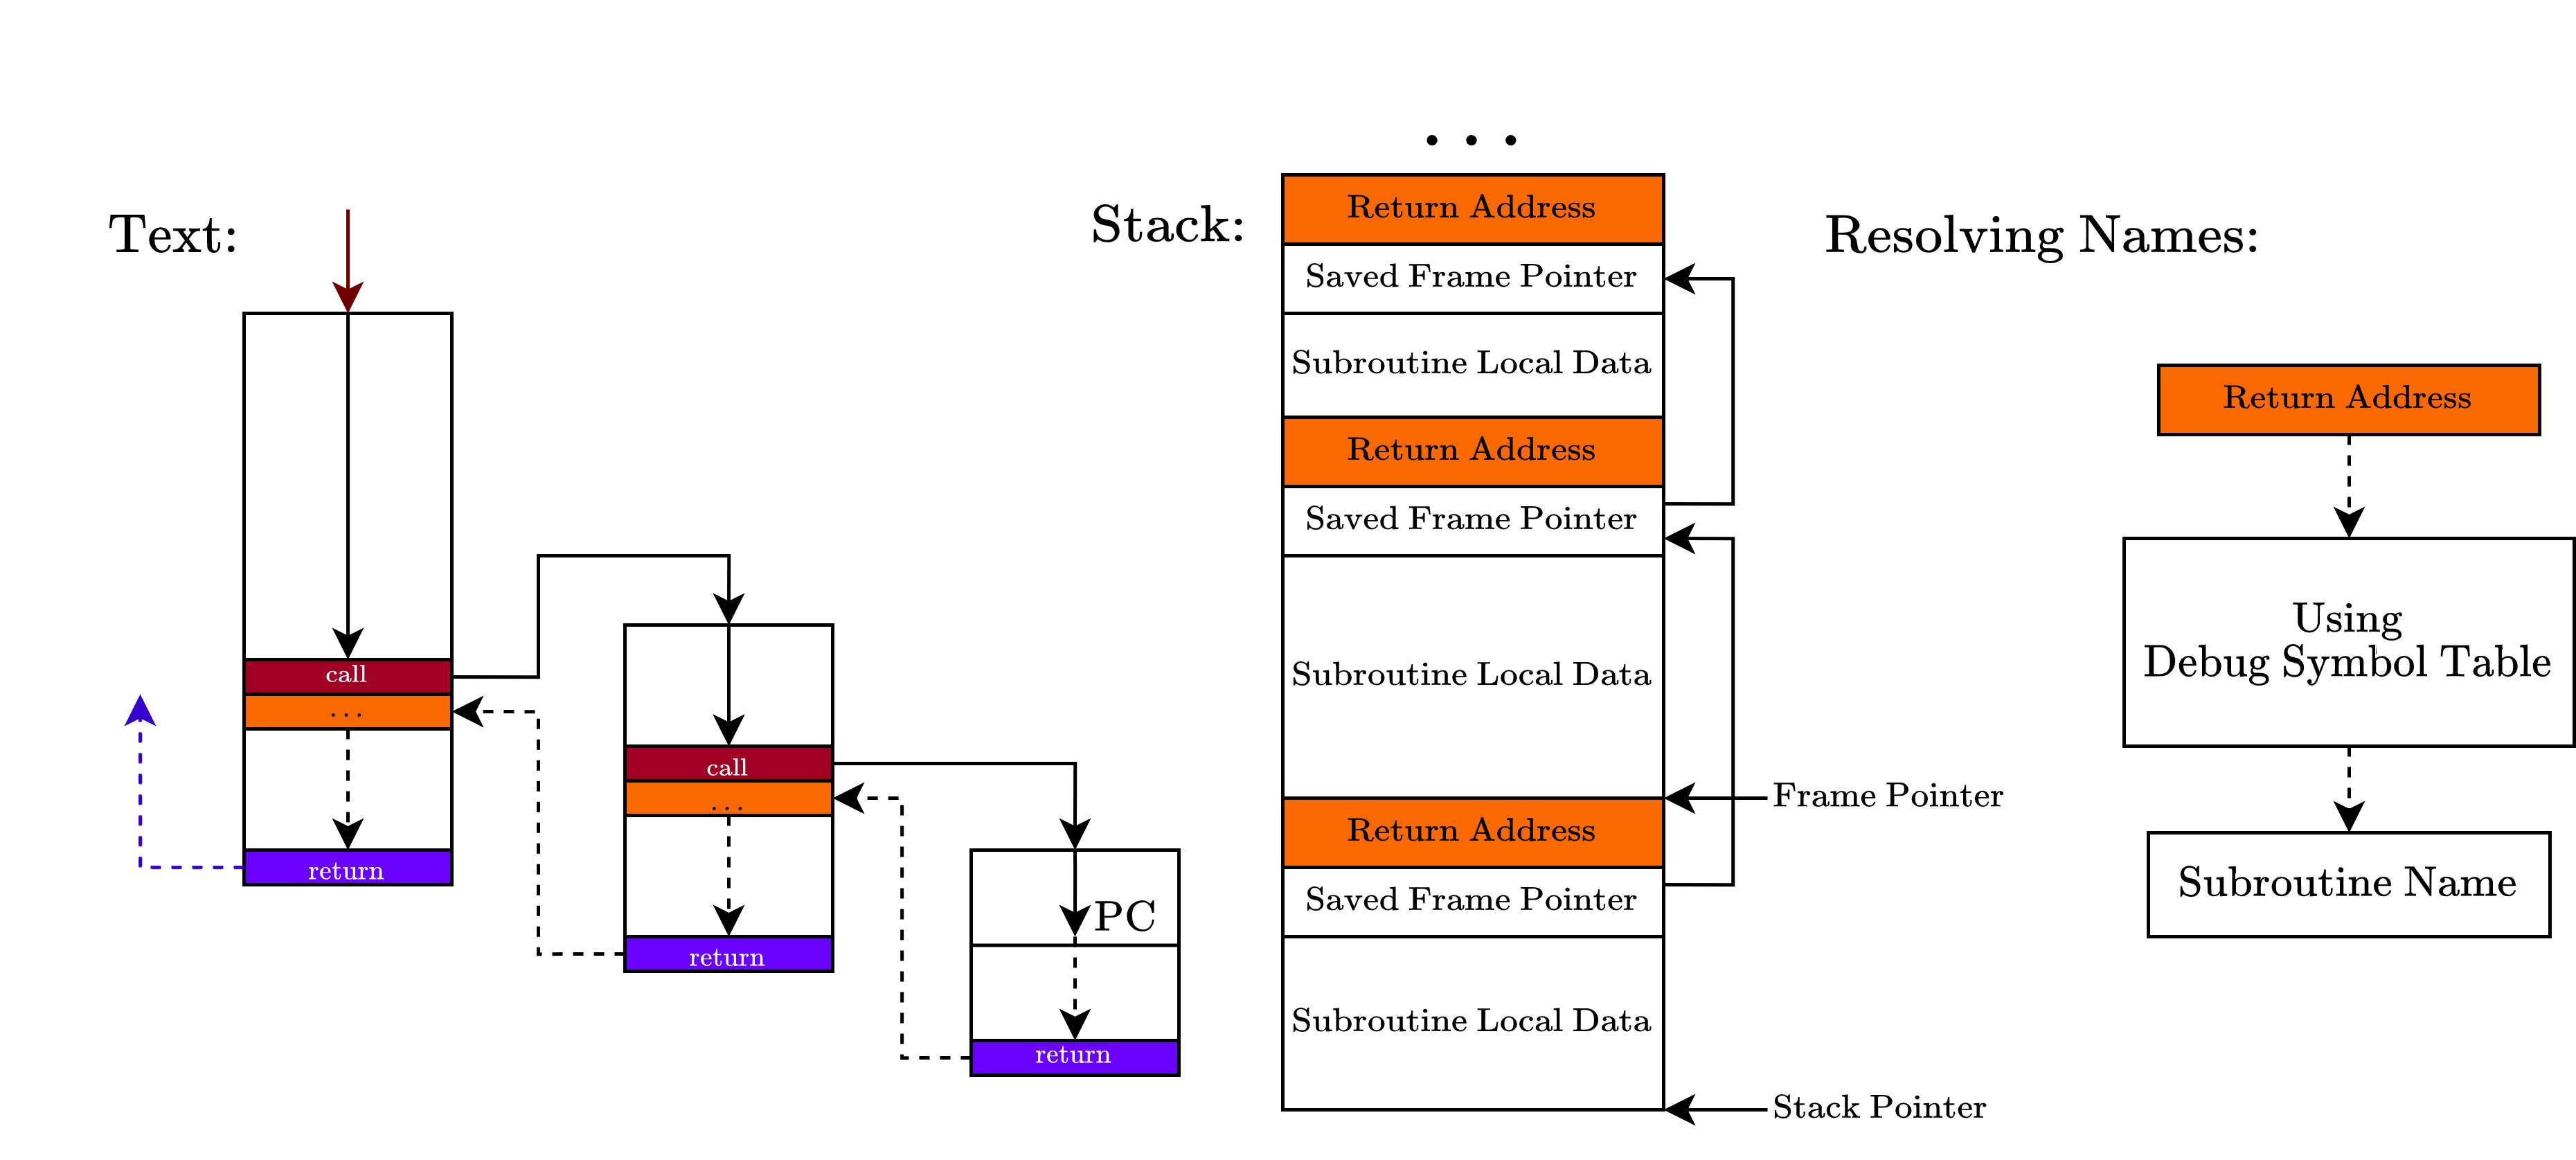
\includegraphics[width=\textwidth]{profiling/images/stack_inspection.drawio.png}
\end{center}
\begin{itemize}
    \item Stack frame layout must conform to a convention that stores frame pointers and return addresses on the stack.
    \item Debug symbols included in the binary (e.g part of the ELF spec) can be used to convert return addresses scraped from the stack into symbols from the source code (function names).
    \item The stack may not easily represent the call structure of a program (inlining, tail call elimination, constant evaluation and propagation)
\end{itemize}


\section{Sampling}
Rather than recording all events, we can reduce overhead by sampling some events.
\begin{tabbox}{prosbox}
    Performance & Fidelity traded against pertubation for reduced overhead in recording events. \\
    Less Pertubation & Fewer interactions with program $\to$ less effect on performance $\to$ less pertubation. \\
\end{tabbox}
\begin{tabbox}{consbox}
    Imperfect & May skip sampling some events (e.g very small functions), but more expensive functions are more likely to be sampled, and we generally care about these more. \\
\end{tabbox}

\subsection{Time-Base Intervals}
We can make use of hardware supported timer interrupts to set timers before using an interrupt to trap and allow the sampler to take control.
\begin{itemize}
    \item Can use CPU \textit{reference cycles} as a proxy metric to time
    \item Hardware clocks are often poorly defined \& vary (i.e variable clock frequencies in modern CPUs, synchronisation of clocks between CPUs)
    \item Easily available \& easy to interpret (ticks $\propto$ time)
\end{itemize}

\subsection{Event-Base Intervals}
A generalisation of time-based intervals (as a clock tick $\to$ time is an event)
\begin{itemize}
    \item Can define in terms of occurrences of an event (e.g function call)
    \item Depending on design, can be accurate / low noise
    \item Can be tricky to interpret as a link to some measure proportional to time is needed (typically we care about execution time)
\end{itemize}

% Quantization Errors
\begin{definitionbox}{Quantisation Errors}
    The resolution of an interval is limited (e.g by clock), but time is continuous. Mapping events to a discrete measure of time can introduce errors \& bias (costs may be attributed to the wrong time \& hence wrong state).
\end{definitionbox}

\subsection{Indirect Tracing}
\begin{definitionbox}{Indirect Tracing}
    We can sample from parts of a program, and infer traces from the structure of the program.
    \\
    \\ For example control flow instructions dominate non-control flow instructions, we could sample from control flow instructions, and then infer event between (non-control flow instructions) (called \textit{basic block counting}), effectively indirectly tracing them.
    \begin{itemize}
        \item Can be used to reduce overhead from tracing
        \item fidelity and accuracy good (depending on the events traced and the indirection used)
    \end{itemize}
\end{definitionbox}

\begin{definitionbox}{Profile}
    A (usually graphical) representation of information relating to the characteristics of a system in terms of resources (quantified) used in certain states.
    \begin{itemize}
        \item An aggregate over a specific metric (e.g a global aggregate if total cache misses, or per event such as cycles per instruction, or cache misses per function)
        \item Information is lost in aggregation
        \item Aggregation has lower overhead than recording all events, so can reduce pertubation 
    \end{itemize}
\end{definitionbox}

\begin{definitionbox}{Flame Graph}
    \begin{center}
        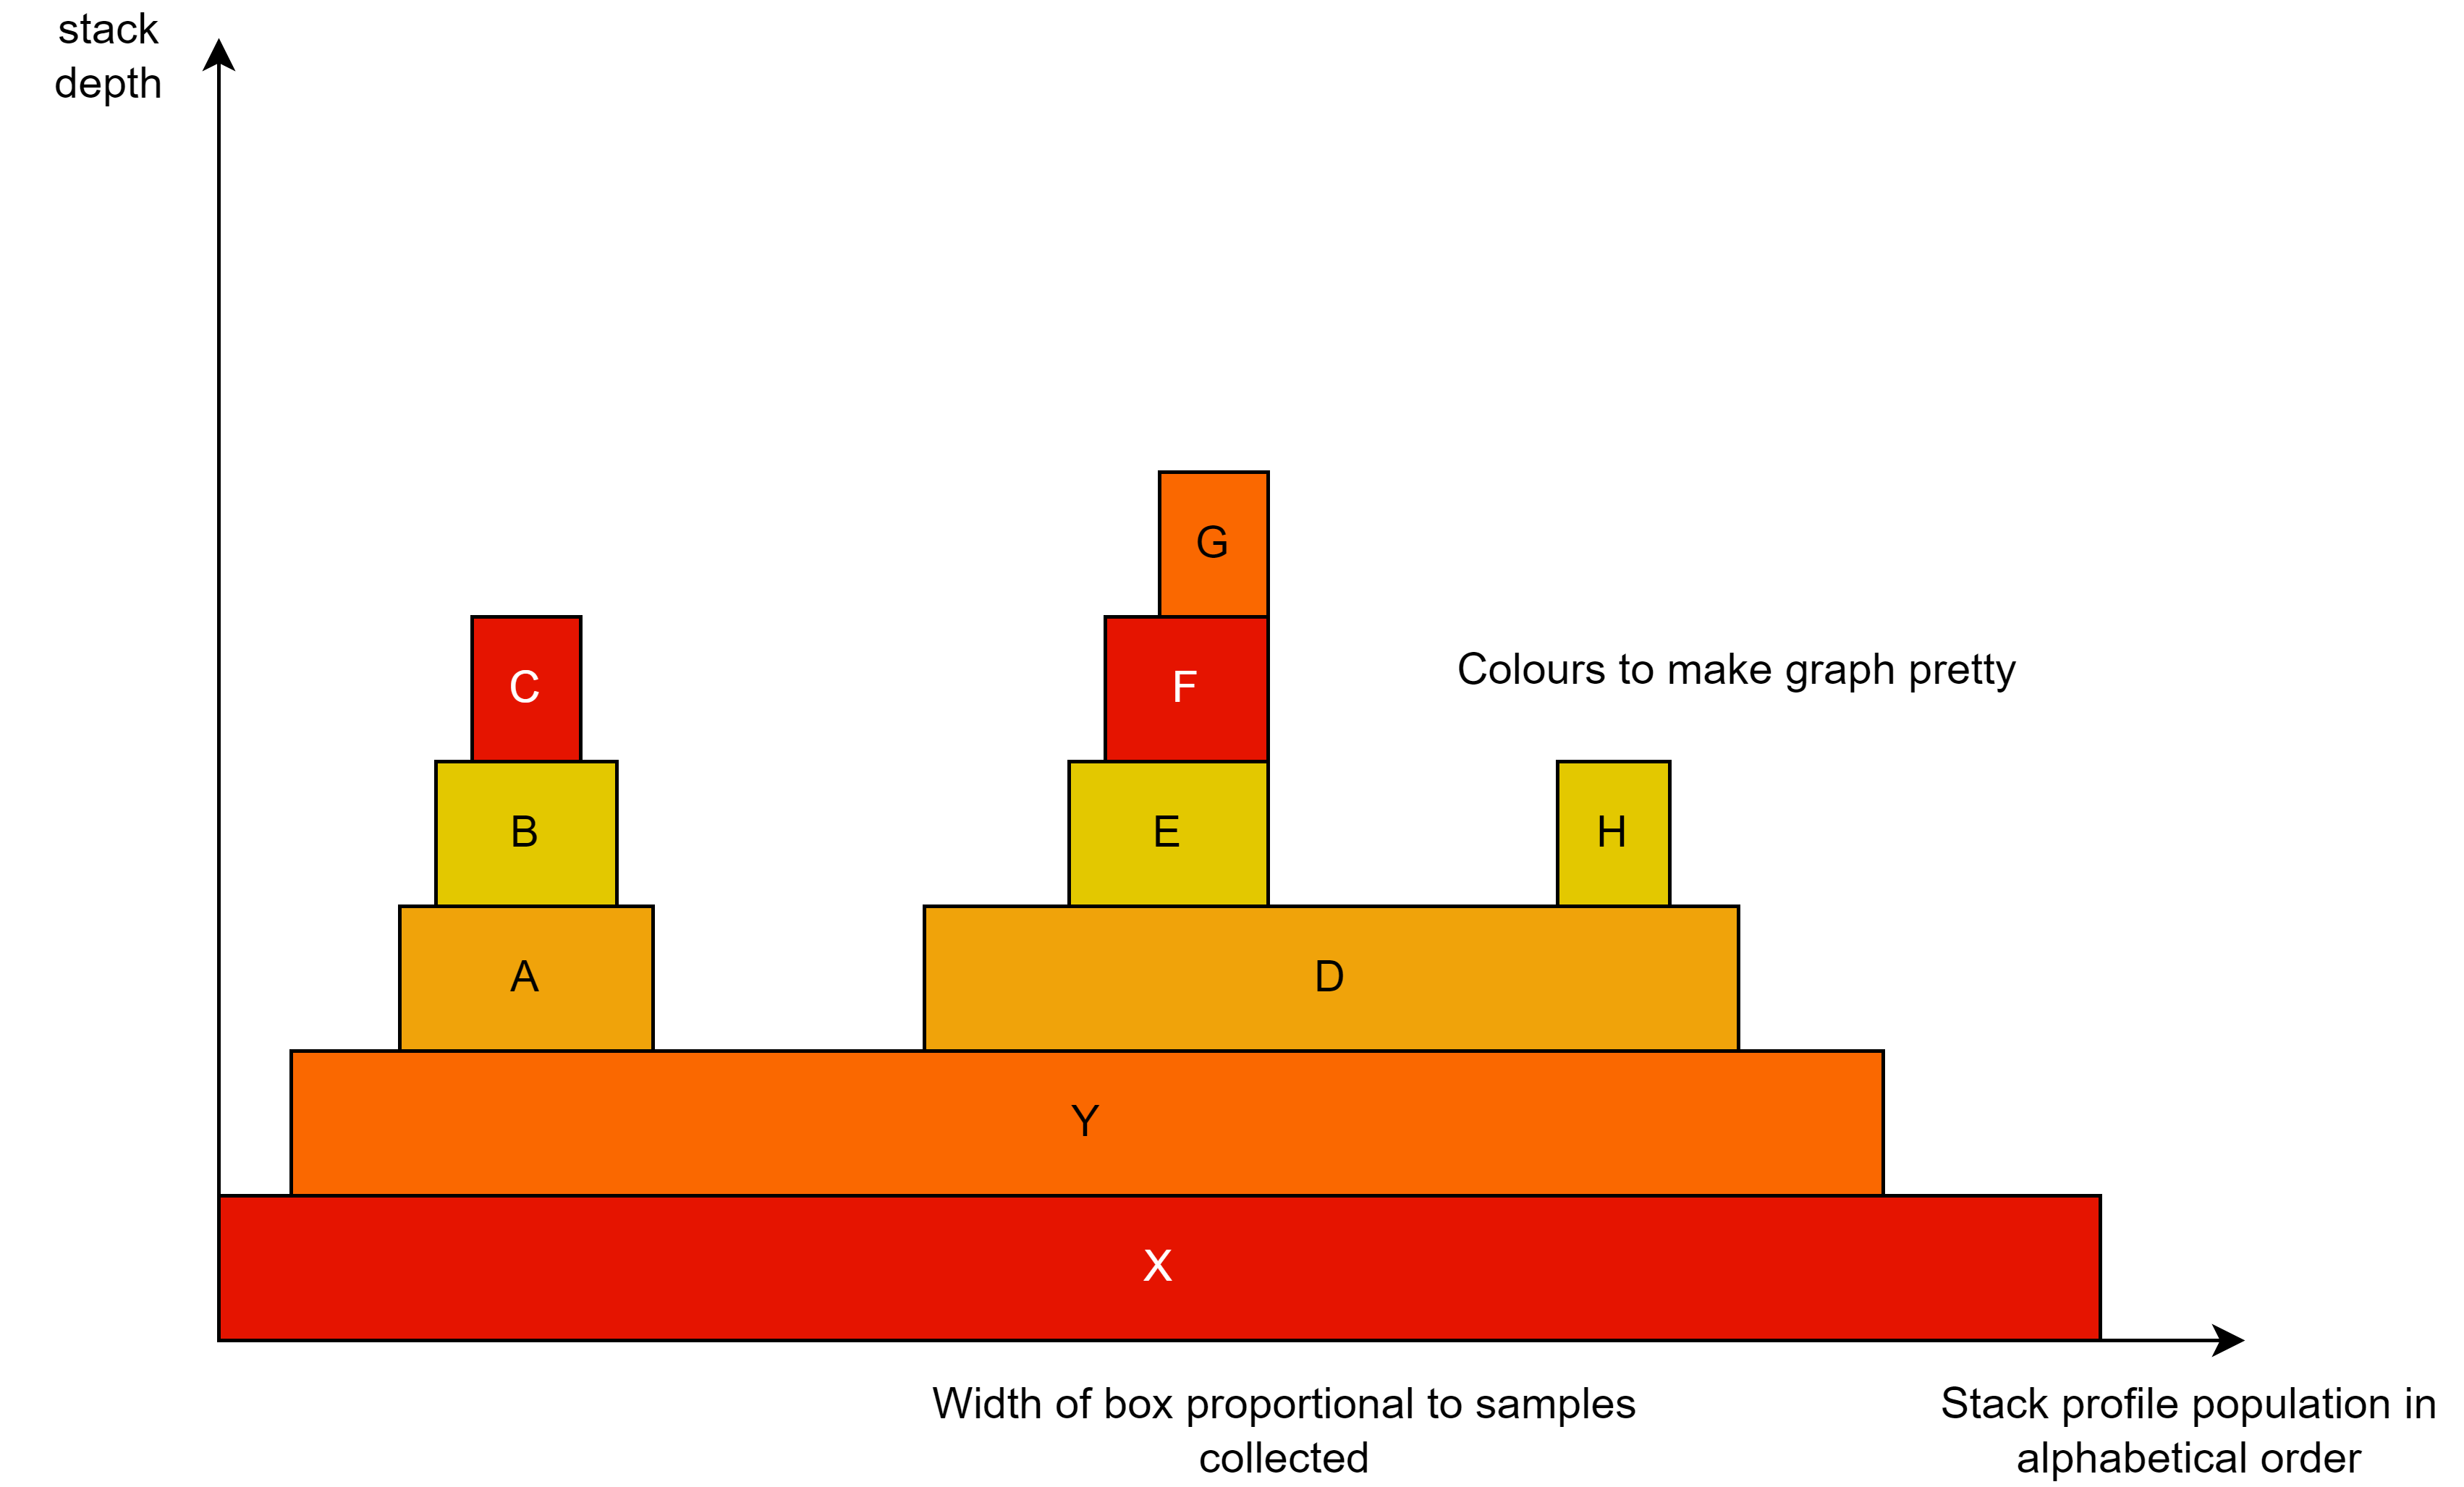
\includegraphics[width=.7\textwidth]{profiling/images/flame_graph.drawio.png}
    \end{center}
\end{definitionbox}

\section{Recording Events}

\begin{definitionbox}{Instrumentation}
    Adding event logging code to a program.
    \begin{tabbox}{prosbox}
        Easily Applicable & No need to extra hardware or OS support. \\
        Flexible & Can implement any kind of logging required. \\
    \end{tabbox}
    \begin{tabbox}{consbox}
        High Overhead & \\
        Perturbation & As part of the program can effect performance \\
    \end{tabbox}
\end{definitionbox}

\subsection{Manual Instrumentation}
Logging using a library (e.g \mintinline{C}{printf} logging)
\begin{tabbox}{prosbox}
    Fine control & Programmer can easily specify exactly where to log what. \\
    Supportless & No need for compiler or hardware support. \\
\end{tabbox}
\begin{tabbox}{consbox}
    High Overhead & \\
    Disable & Need to disable for release builds (recompile without any logging) \\
\end{tabbox}

\subsection{Automatic Instrumentation}
Compiler supported injection of event recording code into a program.
\begin{itemize}
    \item Can be done at source level, or within some intermediate form (e.g injecting into some bytecode)
    \item Can potentially reduce overhead compared with manual instrumentation (compiler instruments at a lower level representation)
\end{itemize}

\subsection{Binary Instrumentation}
Instrumenting an already compiled binary.
\begin{center}
    \begin{tabular}{l p{.8\textwidth}}
        \textbf{Static} & Adding instrumentation directly, overhead can be assessed from the binary. \\
        \textbf{Dynamic} & Adding instrumentation at runtime (works well with JiT) \\
    \end{tabular}
\end{center}


\subsection{Kernel Counters/ Software Performance Counters}
The kernel already has the tools required to collect many kinds of events. These tend to be higher-level OS interactions, rather than microarchitectural events.
For example:
\begin{itemize}
    \item Network packets sent
    \item Virtual memory events (e.g page faults)
    \item Context Switches
    \item Threads spawned
\end{itemize}

\subsection{Emulation}

% Instrumentation
    % Manual
    % Automatic
    % Binary
        % Static
        % Dynamic

% llvm xray
\subsection{Hardware Counters}
Special registers configured to count low-level events as well as intervals (e.g cycles)
\begin{itemize}
    \item Fixed number can be active at runtime
    \item Often buggy / unmaintained / inaccurate (and poorly documented) $\to$ only the most popular counters are trustworthy
\end{itemize}

\section{Perf}
\unfinished

\begin{sidenotebox}{RTFM}
    \href{https://www.intel.com/content/dam/doc/manual/64-ia-32-architectures-optimization-manual.pdf}{Intel 64 and IA-32 Architectures Optimization Reference Manual}.
    \begin{itemize}
        \item Microarchitectural features documented.
        \item Written as an optimisation guide.
        \item Code example can be found in its \href{https://github.com/intel/optimization-manual}{github repo}
    \end{itemize}
\end{sidenotebox}

\section{Microarchitectural bottleneck analysis}
\begin{sidenotebox}{Advanced Computer Architecture}
    A basic understanding of computer architecture is reuired (pipelining, in order, caches, out of order, speculation).
    \\
    \\ The \href{\ACAURL}{60001 - Advanced Computer Architecture} module by Prof Paul Kelly covers this in great depth.
\end{sidenotebox}

\begin{center}
    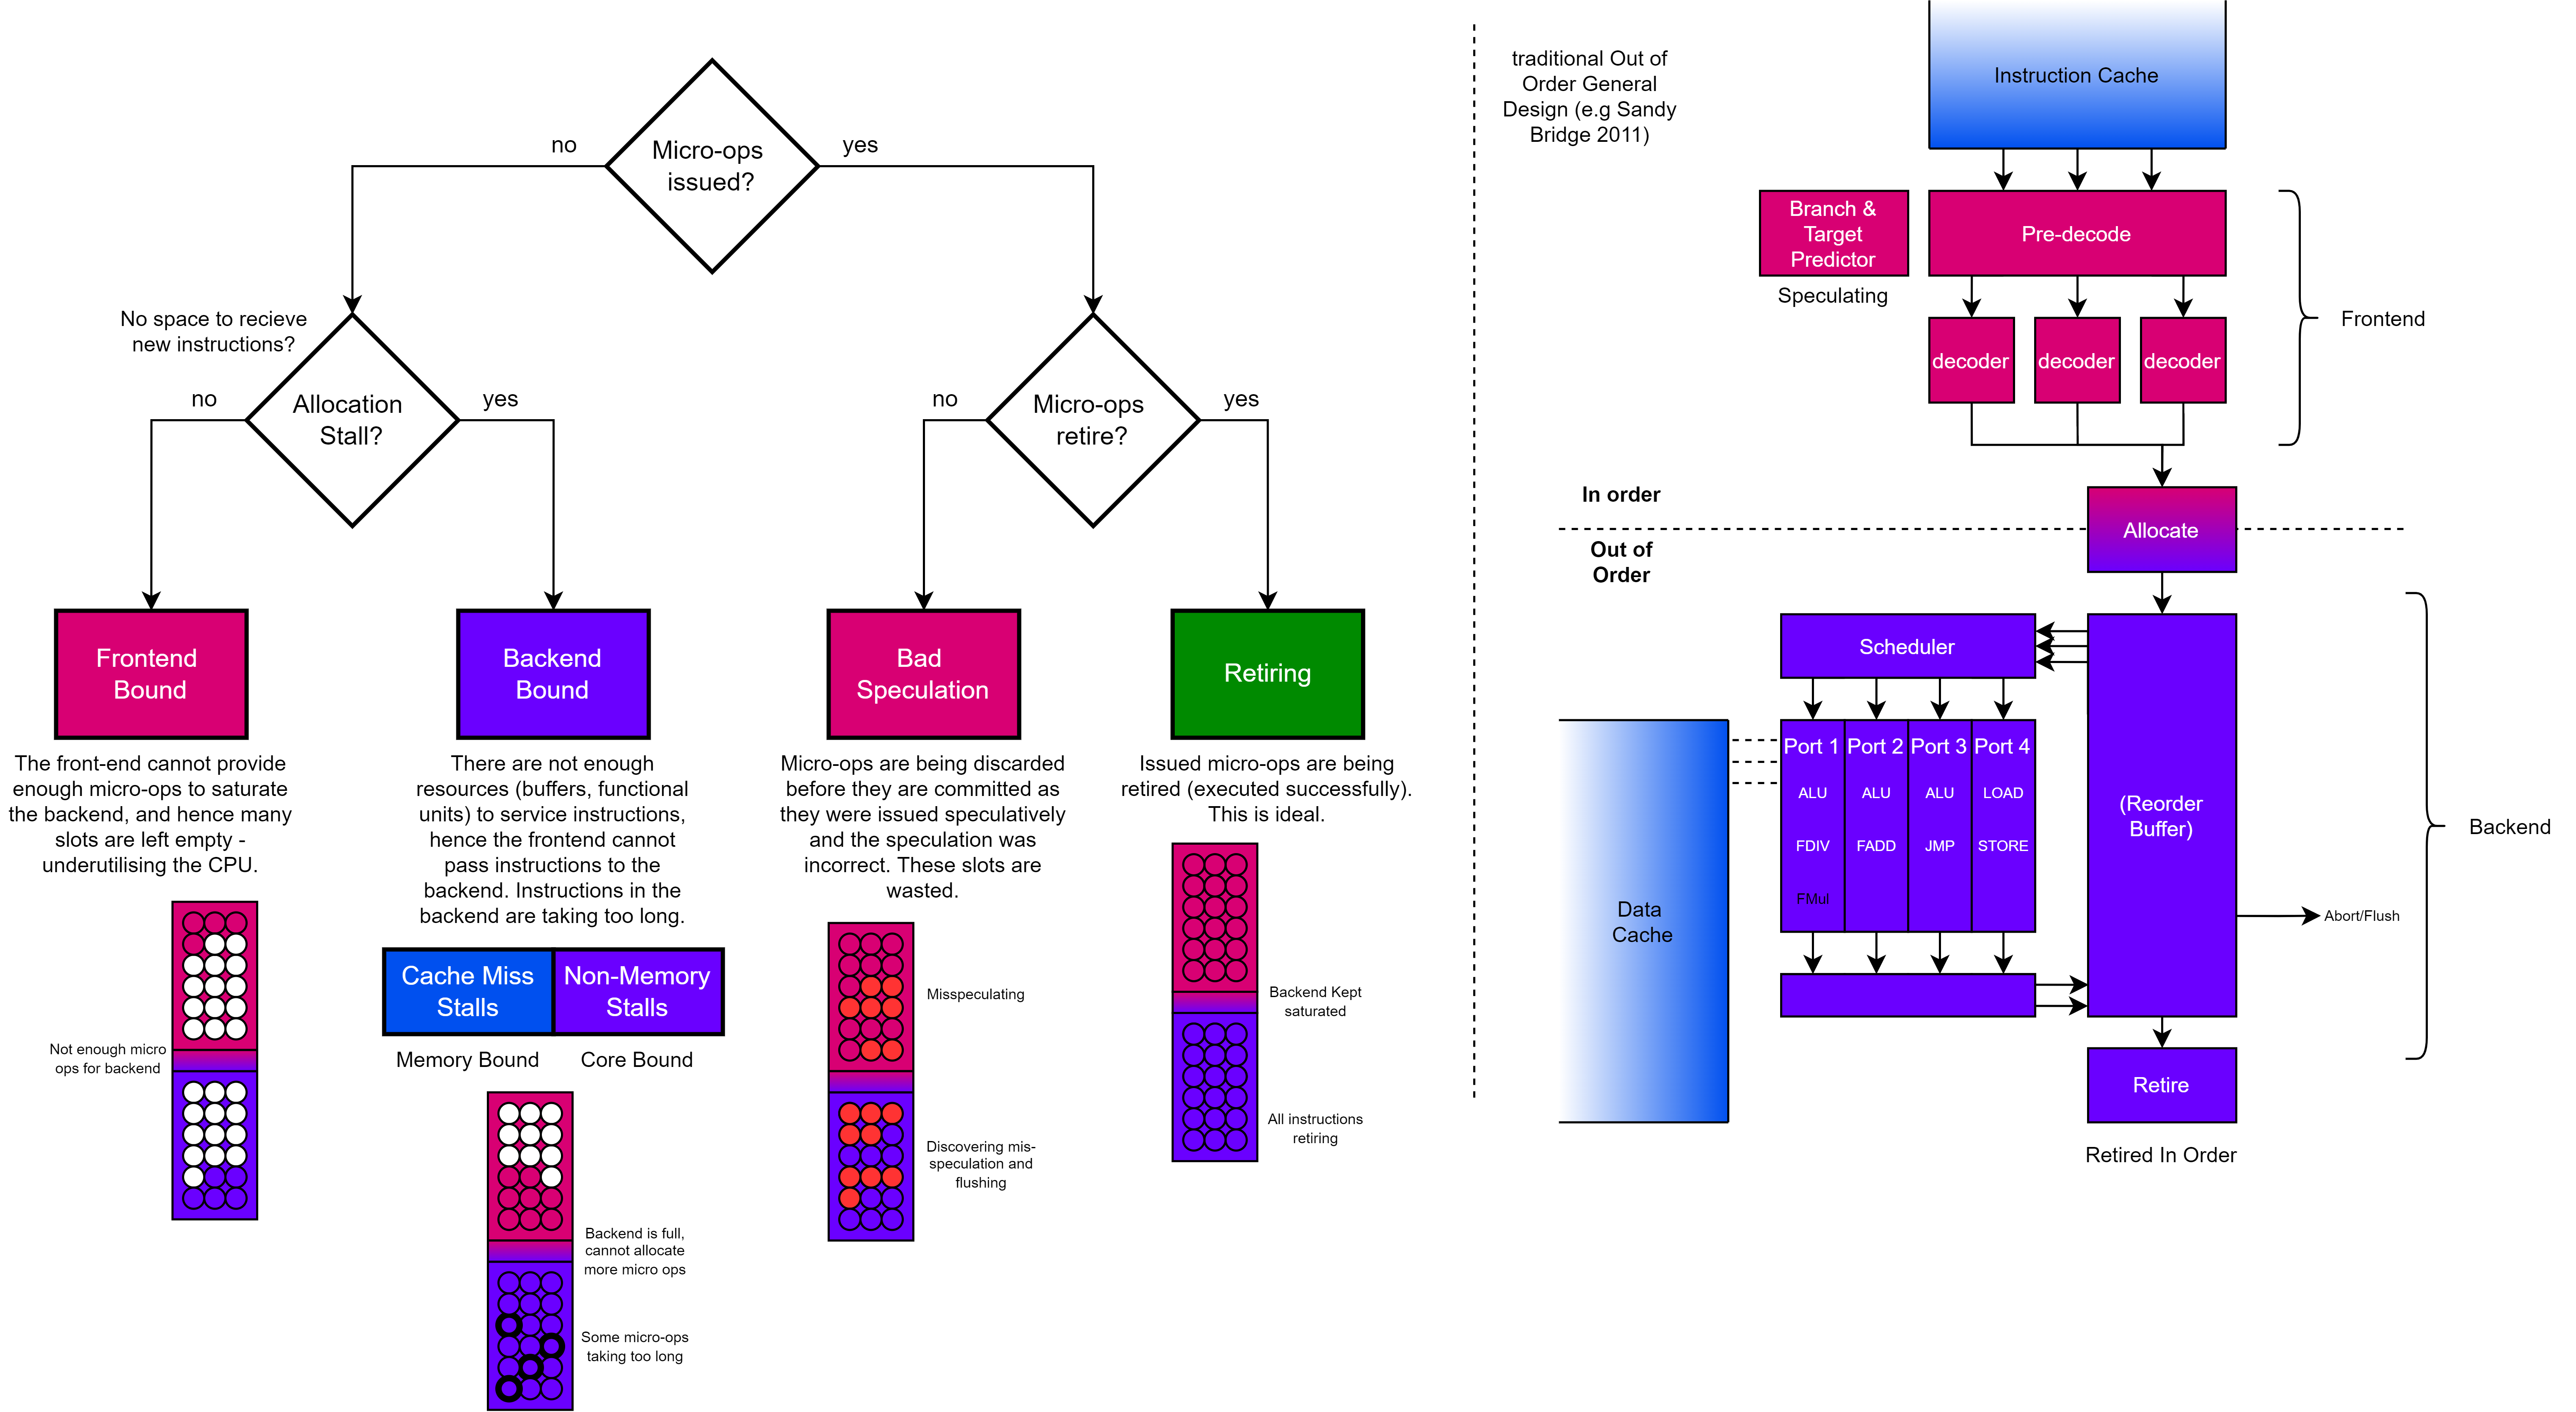
\includegraphics[width=\textwidth]{profiling/images/bottleneck_analysis.drawio.png}
\end{center}
See Intel's \href{https://www.intel.com/content/www/us/en/develop/documentation/vtune-help/top/reference/cpu-metrics-reference.html}{V-Tune performance metrics definitions} for more

\section{Vtune}
\unfinished
